
\documentclass[letterpaper, 11pt]{report}
\usepackage[utf8]{inputenc}
\usepackage{titlesec}
\usepackage{fullpage} % changes the margin
\usepackage{graphicx} %package to manage images
\graphicspath{ {./images/} }

\begin{document}
\begin{titlepage}
\vspace*{0.7in}
\begin{center}
\begin{figure}[htb]
\begin{center}

\includegraphics[width=8cm]{univ_logo}
\end{center}
\end{figure}
\vspace*{0.3in}
\begin{Large}
\textbf{SOEN 6011 : SOFTWARE ENGINEERING PROCESSES} \\
\end{Large}
\vspace*{0.1in}
\begin{Large}
\textbf{SUMMER 2021} \\
\end{Large}
\vspace*{0.9in}
\begin{Large}
\textbf{SUPER CALCULATOR} \\
\end{Large}
\vspace*{0.9in}
\begin{Large} 


\textbf{PROBLEM - 7} \\
 Test Case Review\\
\end{Large}
\vspace*{0.625in}
\rule{80mm}{0.1mm}\\
\vspace*{0.1in}
\begin{large}
Authors \\
\vspace*{0.1in}
Rokeya Begum Keya\\
\vspace*{0.1in}
Kyle Taylor Lange\\
\vspace*{0.1in}
Sijie Min\\
\vspace*{0.1in}
Manimaran Palani\\ 
\vspace*{0.3in}
\date{\normalsize\today} 
\end{large}
\end{center}
\begin{center}
https://www.overleaf.com/project/610304de4e6b8d24f7c781b6\end{center}
\end{titlepage}
\tableofcontents
\newpage
\section*{\centering{PROBLEM 7 - F2: $tan(x)$}}
\normalsize {SOEN 6011 - Summer 2021} \hfill \textbf{Rokeya Begum Keya} \\
\textbf{ Software Engineering Processes}  \hfill \textbf{40183615} \\
\hfill Repository address : https://github.com/Dakatsu/SOEN6011Calculator
\\
\addcontentsline{toc}{section}{a) Test case Review of F5}

\section*{Test case Review of F5}
In this section I have done testing review for the function (F5)- $(y=ab^x)$: \\Developed by Sijie Min. 
\section*{Test Environment}
\item $1$  Eclipse IDE(2020-2021) for Java
\item $2$  JUnit4 framework in Eclipse IDE for
testing\cite{vogella} 
\section*{Testing steps}
\item $1$ Compile the F5 function code in Eclipse.
\item $2$ Give different inputs according to the requirements(P2)
\item $3$ Run the JUnit4 to check the output
\item $4$ verified the output 
\item I was unable to test her function manually in the SuperCalculator since she did not integrated her function in SuperCalculator.java and the button does not use her function.
\section*{Result of JUnit4 Testing}
\begin{center}
\begin{tabular}{ |c|c|c| }
\hline
Requirements & Details & Output \\
 \hline
 R5-R1 & when X = "0" & Pass \\ 
 R5-R2 & check Positive and Negative number & Pass \\ 
 R5-R3 & check multiplication & pass \\ 
 \hline
\end{tabular}
\end{center}
\item Result of the test cases are given based on the requirements. 
\pagebreak

\section*{\centering{PROBLEM 7 - F3: Hyperbolic Sine, $sinh(x)$}}
\normalsize {SOEN 6011 - Summer 2021} \hfill \textbf{Kyle Taylor Lange} \\
\textbf{ Software Engineering Processes}  \hfill \textbf{27627696} \\
\hfill Repository address : https://github.com/Dakatsu/SOEN6011Calculator
\\
\addcontentsline{toc}{section}{b) Test case Review of F7}

\section*{Test case Review of F7}
The JUnit tests that Manimaran Palani created to test his power function have Javadoc comments that list the exact specification the unit test is built for. All but one of his unit tests are entirely atomic, with only the input validation having multiple assertion statements. I ran the tests in Eclipse, and all of them passed. \\
\begin{figure}[htb]
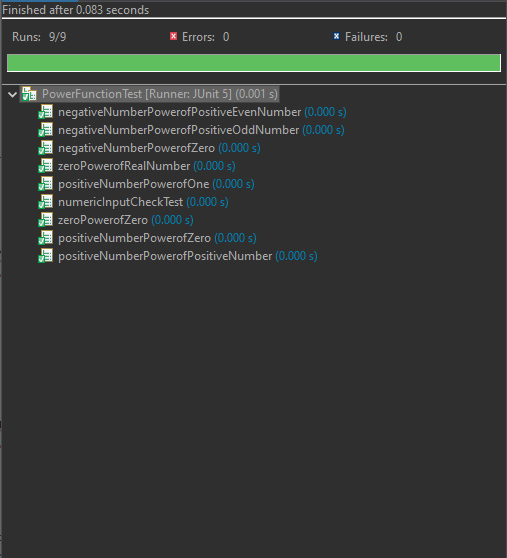
\includegraphics[width=0.5\textwidth]{TestF7}
\centering
\caption{Results of the JUnit tests located in PowerFunctionTest.java}
\end{figure} \\
\pagebreak
I then proceeded to do a manual test of the function within the calculator application itself, calculating multiple values in Microsoft Excel before testing the outputs when entered into the calculator. Integer values were all accurate to the calculations, while numbers with decimals varied in accuracy. \\
\begin{figure}[htb]
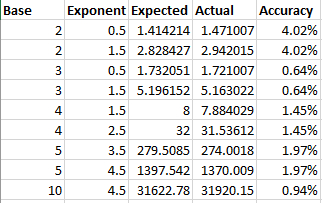
\includegraphics[width=0.5\textwidth]{ErrorF7}
\centering
\caption{Percentage error values computed against select non-integer inputs.}
\end{figure} \\\\

\pagebreak

\section*{\centering{PROBLEM 7 - F5:\(y=ab^x\)}}
\normalsize {SOEN 6011 - Summer 2021} \hfill \textbf{Sijie Min} \\
\textbf{ Software Engineering Processes}  \hfill \textbf{40152234} \\
\hfill Repository address : https://github.com/Dakatsu/SOEN6011Calculator
\\
\addcontentsline{toc}{section}{c) Test case Review of F2}
\section*{Test case Review of F2}

\\\\The test is completed in eclipse with JUnit4, and the corresponding test java file is run as JUnit Test. For the requirements mentioned in problem2, there are corresponding test cases in the test code. All test cases have passed, and it is possible for requirementF2-R6 It can be seen that the test is successful through the running time of the test.

\begin{figure}[htp]
    \centering
    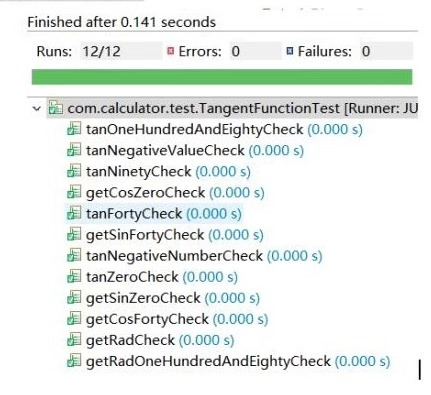
\includegraphics[width=16cm]{SOEN_6011-Problem-7/F5P7.jpg}
    \caption{Test case review of F2}
    \label{fig:galaxy}
\end{figure}
 \begin{center} 
\end{center}

\pagebreak

\section*{\centering{PROBLEM 7 - F7 : \(x^y\)}}
\normalsize {SOEN 6011 - Summer 2021} \hfill \textbf{Manimaran Palani} \\
\textbf{ Software Engineering Processes}  \hfill \textbf{40167543} \\
\hfill Repository address : https://github.com/Dakatsu/SOEN6011Calculator
\\
\addcontentsline{toc}{section}{d) Test case Review of F3}
\section*{Test case Review of F3}
This sections presents the test case review of a  Transcendental function (F3) - $sinh(x)$: \\Developed by Kyle Taylor Lange.
\section*{Test Suite}
Junit test cases\cite{vogella} are performed with Junit4 framework.
\\\\
As per Java coding standards, the JUnit test cases are created and maintained in a separate folder structure to perform the testing process with zero impact on code section.
\section*{Test Case Results}
\textbf{SinhLibrariesTest.java} file was run with Junit4 suite and obtained the below results.
\\
\begin{figure}[htb]
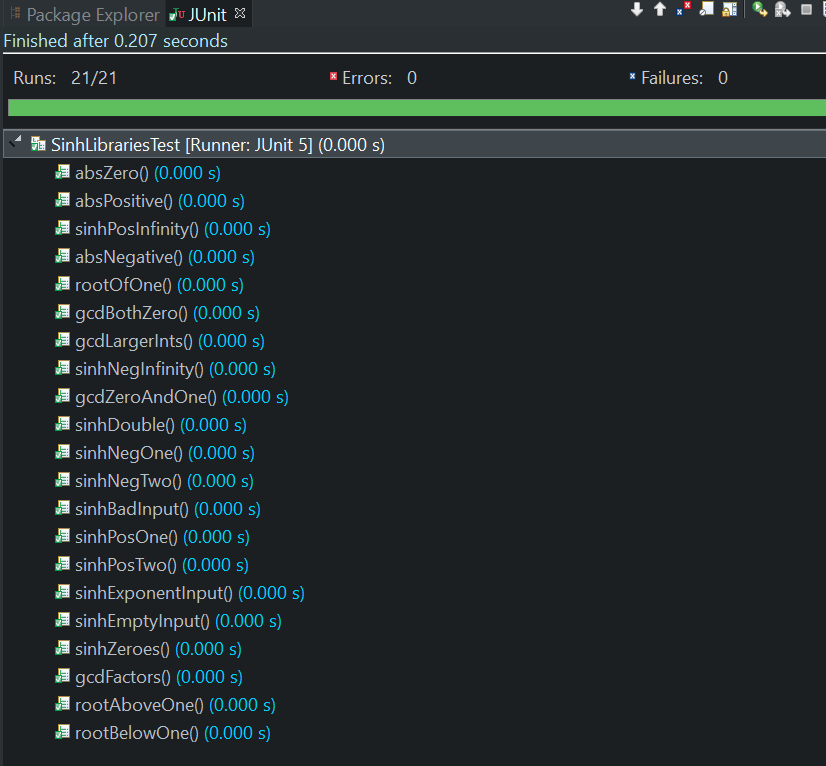
\includegraphics[width=0.5\textwidth]{TestCases_Review_Results_F3}
\centering
\caption{Junit test cases are passed in JUnit[4] in Eclipse IDE}
\end{figure}
\begin{thebibliography}{}
\bibitem{vogella} 
vogella. Unit Testing with JUnit. 2007. 
\\\texttt{https://www.vogella.com/tutorials/JUnit/article.html}
\end{thebibliography}
\end{document}
